\section{APPENDIX}
\subsection*{A. Work organization chart}
\begin{figure}[H]
    \centering
    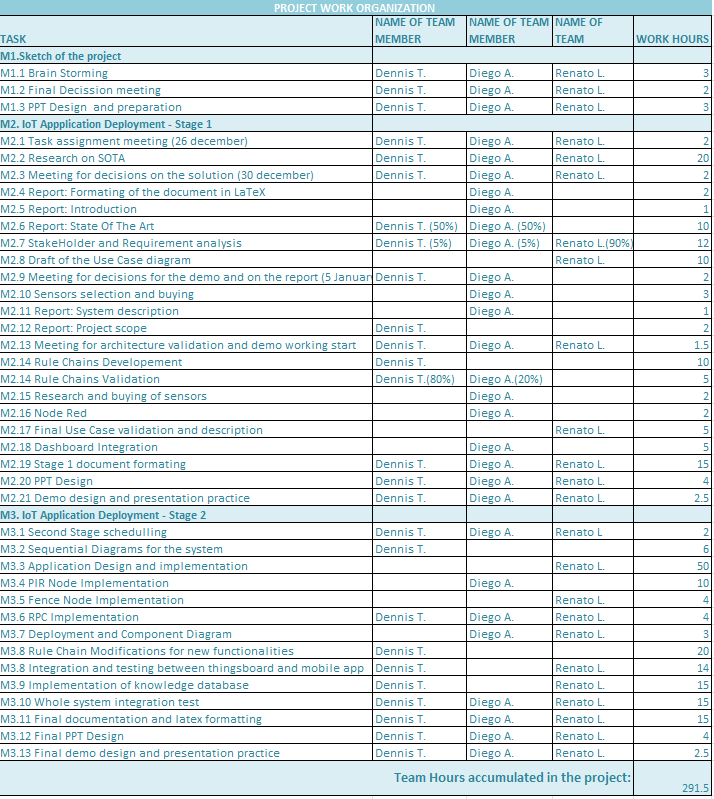
\includegraphics[width=1\textwidth]{./images/Tasks.png}
    \caption{Tasks for the first stage of the project}
    \label{fig:tasks}
\end{figure}

\subsection*{B. Mosquitto MQTT alarms messages for mobile application notification}
JSON message sent to UPM/MIoT/ARS/RiskSystem/alarms/PresenceDetected topic to indicate presence in the nearby area of the fence.
\lstinputlisting[caption={JSON message for Presence Alarm}, label={lst:presenceAlarm}]{code/presenceAlarmMQTT.json}

JSON message sent to UPM/MIoT/ARS/RiskSystem/alarms/FireHazard topic to indicate the possible presence in the nearby area of a wild fire.
\lstinputlisting[caption={JSON message for Fire Hazard Alarm}, label={lst:presenceAlarm}]{code/fireHazardAlarmMQTT.json}
\clearpage
JSON message sent to UPM/MIoT/ARS/RiskSystem/alarms/FenceTrespassed topic to indicate the possible trespassed of a fence.
\lstinputlisting[caption={JSON message for Fence Trespassed Alarm}, label={lst:presenceAlarm}]{code/fenceTrespassedAlarmMQTT.json}

JSON message sent to the rest of the topics to indicate the status of an specific alarm and the originator node.
\lstinputlisting[caption={JSON message for the other alarms}, label={lst:presenceAlarm}]{code/generalAlarmMQTT.json}

